%%%%%%%% ICML 2025 EXAMPLE LATEX SUBMISSION FILE %%%%%%%%%%%%%%%%%

\documentclass{article}

% Recommended, but optional, packages for figures and better typesetting:
\usepackage{microtype}
\usepackage{graphicx}
\usepackage{subfigure}
% \usepackage{algorithm2e}
\usepackage{booktabs} % for professional tables

% hyperref makes hyperlinks in the resulting PDF.
% If your build breaks (sometimes temporarily if a hyperlink spans a page)
% please comment out the following usepackage line and replace
% \usepackage{icml2025} with \usepackage[nohyperref]{icml2025} above.
\usepackage{hyperref}
\usepackage{arydshln}

% Attempt to make hyperref and algorithmic work together better:
\newcommand{\theHalgorithm}{\arabic{algorithm}}

% Use the following line for the initial blind version submitted for review:
\usepackage{icml2025}

% If accepted, instead use the following line for the camera-ready submission:
% \usepackage[accepted]{icml2025}

% For theorems and such
\usepackage{amsmath}
\usepackage{amssymb}
\usepackage{mathtools}
\usepackage{amsthm}

% if you use cleveref..
\usepackage[capitalize,noabbrev]{cleveref}

%%%%% NEW MATH DEFINITIONS %%%%%

\usepackage{amsmath,amsfonts,bm}

% Mark sections of captions for referring to divisions of figures
\newcommand{\figleft}{{\em (Left)}}
\newcommand{\figcenter}{{\em (Center)}}
\newcommand{\figright}{{\em (Right)}}
\newcommand{\figtop}{{\em (Top)}}
\newcommand{\figbottom}{{\em (Bottom)}}
\newcommand{\captiona}{{\em (a)}}
\newcommand{\captionb}{{\em (b)}}
\newcommand{\captionc}{{\em (c)}}
\newcommand{\captiond}{{\em (d)}}

% Highlight a newly defined term
\newcommand{\newterm}[1]{{\bf #1}}


% Figure reference, lower-case.
\def\figref#1{figure~\ref{#1}}
% Figure reference, capital. For start of sentence
\def\Figref#1{Figure~\ref{#1}}
\def\twofigref#1#2{figures \ref{#1} and \ref{#2}}
\def\quadfigref#1#2#3#4{figures \ref{#1}, \ref{#2}, \ref{#3} and \ref{#4}}
% Section reference, lower-case.
\def\secref#1{section~\ref{#1}}
% Section reference, capital.
\def\Secref#1{Section~\ref{#1}}
% Reference to two sections.
\def\twosecrefs#1#2{sections \ref{#1} and \ref{#2}}
% Reference to three sections.
\def\secrefs#1#2#3{sections \ref{#1}, \ref{#2} and \ref{#3}}
% Reference to an equation, lower-case.
\def\eqref#1{equation~\ref{#1}}
% Reference to an equation, upper case
\def\Eqref#1{Equation~\ref{#1}}
% A raw reference to an equation---avoid using if possible
\def\plaineqref#1{\ref{#1}}
% Reference to a chapter, lower-case.
\def\chapref#1{chapter~\ref{#1}}
% Reference to an equation, upper case.
\def\Chapref#1{Chapter~\ref{#1}}
% Reference to a range of chapters
\def\rangechapref#1#2{chapters\ref{#1}--\ref{#2}}
% Reference to an algorithm, lower-case.
\def\algref#1{algorithm~\ref{#1}}
% Reference to an algorithm, upper case.
\def\Algref#1{Algorithm~\ref{#1}}
\def\twoalgref#1#2{algorithms \ref{#1} and \ref{#2}}
\def\Twoalgref#1#2{Algorithms \ref{#1} and \ref{#2}}
% Reference to a part, lower case
\def\partref#1{part~\ref{#1}}
% Reference to a part, upper case
\def\Partref#1{Part~\ref{#1}}
\def\twopartref#1#2{parts \ref{#1} and \ref{#2}}

\def\ceil#1{\lceil #1 \rceil}
\def\floor#1{\lfloor #1 \rfloor}
\def\1{\bm{1}}
\newcommand{\train}{\mathcal{D}}
\newcommand{\valid}{\mathcal{D_{\mathrm{valid}}}}
\newcommand{\test}{\mathcal{D_{\mathrm{test}}}}

\def\eps{{\epsilon}}


% Random variables
\def\reta{{\textnormal{$\eta$}}}
\def\ra{{\textnormal{a}}}
\def\rb{{\textnormal{b}}}
\def\rc{{\textnormal{c}}}
\def\rd{{\textnormal{d}}}
\def\re{{\textnormal{e}}}
\def\rf{{\textnormal{f}}}
\def\rg{{\textnormal{g}}}
\def\rh{{\textnormal{h}}}
\def\ri{{\textnormal{i}}}
\def\rj{{\textnormal{j}}}
\def\rk{{\textnormal{k}}}
\def\rl{{\textnormal{l}}}
% rm is already a command, just don't name any random variables m
\def\rn{{\textnormal{n}}}
\def\ro{{\textnormal{o}}}
\def\rp{{\textnormal{p}}}
\def\rq{{\textnormal{q}}}
\def\rr{{\textnormal{r}}}
\def\rs{{\textnormal{s}}}
\def\rt{{\textnormal{t}}}
\def\ru{{\textnormal{u}}}
\def\rv{{\textnormal{v}}}
\def\rw{{\textnormal{w}}}
\def\rx{{\textnormal{x}}}
\def\ry{{\textnormal{y}}}
\def\rz{{\textnormal{z}}}

% Random vectors
\def\rvepsilon{{\mathbf{\epsilon}}}
\def\rvtheta{{\mathbf{\theta}}}
\def\rva{{\mathbf{a}}}
\def\rvb{{\mathbf{b}}}
\def\rvc{{\mathbf{c}}}
\def\rvd{{\mathbf{d}}}
\def\rve{{\mathbf{e}}}
\def\rvf{{\mathbf{f}}}
\def\rvg{{\mathbf{g}}}
\def\rvh{{\mathbf{h}}}
\def\rvu{{\mathbf{i}}}
\def\rvj{{\mathbf{j}}}
\def\rvk{{\mathbf{k}}}
\def\rvl{{\mathbf{l}}}
\def\rvm{{\mathbf{m}}}
\def\rvn{{\mathbf{n}}}
\def\rvo{{\mathbf{o}}}
\def\rvp{{\mathbf{p}}}
\def\rvq{{\mathbf{q}}}
\def\rvr{{\mathbf{r}}}
\def\rvs{{\mathbf{s}}}
\def\rvt{{\mathbf{t}}}
\def\rvu{{\mathbf{u}}}
\def\rvv{{\mathbf{v}}}
\def\rvw{{\mathbf{w}}}
\def\rvx{{\mathbf{x}}}
\def\rvy{{\mathbf{y}}}
\def\rvz{{\mathbf{z}}}

% Elements of random vectors
\def\erva{{\textnormal{a}}}
\def\ervb{{\textnormal{b}}}
\def\ervc{{\textnormal{c}}}
\def\ervd{{\textnormal{d}}}
\def\erve{{\textnormal{e}}}
\def\ervf{{\textnormal{f}}}
\def\ervg{{\textnormal{g}}}
\def\ervh{{\textnormal{h}}}
\def\ervi{{\textnormal{i}}}
\def\ervj{{\textnormal{j}}}
\def\ervk{{\textnormal{k}}}
\def\ervl{{\textnormal{l}}}
\def\ervm{{\textnormal{m}}}
\def\ervn{{\textnormal{n}}}
\def\ervo{{\textnormal{o}}}
\def\ervp{{\textnormal{p}}}
\def\ervq{{\textnormal{q}}}
\def\ervr{{\textnormal{r}}}
\def\ervs{{\textnormal{s}}}
\def\ervt{{\textnormal{t}}}
\def\ervu{{\textnormal{u}}}
\def\ervv{{\textnormal{v}}}
\def\ervw{{\textnormal{w}}}
\def\ervx{{\textnormal{x}}}
\def\ervy{{\textnormal{y}}}
\def\ervz{{\textnormal{z}}}

% Random matrices
\def\rmA{{\mathbf{A}}}
\def\rmB{{\mathbf{B}}}
\def\rmC{{\mathbf{C}}}
\def\rmD{{\mathbf{D}}}
\def\rmE{{\mathbf{E}}}
\def\rmF{{\mathbf{F}}}
\def\rmG{{\mathbf{G}}}
\def\rmH{{\mathbf{H}}}
\def\rmI{{\mathbf{I}}}
\def\rmJ{{\mathbf{J}}}
\def\rmK{{\mathbf{K}}}
\def\rmL{{\mathbf{L}}}
\def\rmM{{\mathbf{M}}}
\def\rmN{{\mathbf{N}}}
\def\rmO{{\mathbf{O}}}
\def\rmP{{\mathbf{P}}}
\def\rmQ{{\mathbf{Q}}}
\def\rmR{{\mathbf{R}}}
\def\rmS{{\mathbf{S}}}
\def\rmT{{\mathbf{T}}}
\def\rmU{{\mathbf{U}}}
\def\rmV{{\mathbf{V}}}
\def\rmW{{\mathbf{W}}}
\def\rmX{{\mathbf{X}}}
\def\rmY{{\mathbf{Y}}}
\def\rmZ{{\mathbf{Z}}}

% Elements of random matrices
\def\ermA{{\textnormal{A}}}
\def\ermB{{\textnormal{B}}}
\def\ermC{{\textnormal{C}}}
\def\ermD{{\textnormal{D}}}
\def\ermE{{\textnormal{E}}}
\def\ermF{{\textnormal{F}}}
\def\ermG{{\textnormal{G}}}
\def\ermH{{\textnormal{H}}}
\def\ermI{{\textnormal{I}}}
\def\ermJ{{\textnormal{J}}}
\def\ermK{{\textnormal{K}}}
\def\ermL{{\textnormal{L}}}
\def\ermM{{\textnormal{M}}}
\def\ermN{{\textnormal{N}}}
\def\ermO{{\textnormal{O}}}
\def\ermP{{\textnormal{P}}}
\def\ermQ{{\textnormal{Q}}}
\def\ermR{{\textnormal{R}}}
\def\ermS{{\textnormal{S}}}
\def\ermT{{\textnormal{T}}}
\def\ermU{{\textnormal{U}}}
\def\ermV{{\textnormal{V}}}
\def\ermW{{\textnormal{W}}}
\def\ermX{{\textnormal{X}}}
\def\ermY{{\textnormal{Y}}}
\def\ermZ{{\textnormal{Z}}}

% Vectors
\def\vzero{{\bm{0}}}
\def\vone{{\bm{1}}}
\def\vmu{{\bm{\mu}}}
\def\vtheta{{\bm{\theta}}}
\def\va{{\bm{a}}}
\def\vb{{\bm{b}}}
\def\vc{{\bm{c}}}
\def\vd{{\bm{d}}}
\def\ve{{\bm{e}}}
\def\vf{{\bm{f}}}
\def\vg{{\bm{g}}}
\def\vh{{\bm{h}}}
\def\vi{{\bm{i}}}
\def\vj{{\bm{j}}}
\def\vk{{\bm{k}}}
\def\vl{{\bm{l}}}
\def\vm{{\bm{m}}}
\def\vn{{\bm{n}}}
\def\vo{{\bm{o}}}
\def\vp{{\bm{p}}}
\def\vq{{\bm{q}}}
\def\vr{{\bm{r}}}
\def\vs{{\bm{s}}}
\def\vt{{\bm{t}}}
\def\vu{{\bm{u}}}
\def\vv{{\bm{v}}}
\def\vw{{\bm{w}}}
\def\vx{{\bm{x}}}
\def\vy{{\bm{y}}}
\def\vz{{\bm{z}}}

% Elements of vectors
\def\evalpha{{\alpha}}
\def\evbeta{{\beta}}
\def\evepsilon{{\epsilon}}
\def\evlambda{{\lambda}}
\def\evomega{{\omega}}
\def\evmu{{\mu}}
\def\evpsi{{\psi}}
\def\evsigma{{\sigma}}
\def\evtheta{{\theta}}
\def\eva{{a}}
\def\evb{{b}}
\def\evc{{c}}
\def\evd{{d}}
\def\eve{{e}}
\def\evf{{f}}
\def\evg{{g}}
\def\evh{{h}}
\def\evi{{i}}
\def\evj{{j}}
\def\evk{{k}}
\def\evl{{l}}
\def\evm{{m}}
\def\evn{{n}}
\def\evo{{o}}
\def\evp{{p}}
\def\evq{{q}}
\def\evr{{r}}
\def\evs{{s}}
\def\evt{{t}}
\def\evu{{u}}
\def\evv{{v}}
\def\evw{{w}}
\def\evx{{x}}
\def\evy{{y}}
\def\evz{{z}}

% Matrix
\def\mA{{\bm{A}}}
\def\mB{{\bm{B}}}
\def\mC{{\bm{C}}}
\def\mD{{\bm{D}}}
\def\mE{{\bm{E}}}
\def\mF{{\bm{F}}}
\def\mG{{\bm{G}}}
\def\mH{{\bm{H}}}
\def\mI{{\bm{I}}}
\def\mJ{{\bm{J}}}
\def\mK{{\bm{K}}}
\def\mL{{\bm{L}}}
\def\mM{{\bm{M}}}
\def\mN{{\bm{N}}}
\def\mO{{\bm{O}}}
\def\mP{{\bm{P}}}
\def\mQ{{\bm{Q}}}
\def\mR{{\bm{R}}}
\def\mS{{\bm{S}}}
\def\mT{{\bm{T}}}
\def\mU{{\bm{U}}}
\def\mV{{\bm{V}}}
\def\mW{{\bm{W}}}
\def\mX{{\bm{X}}}
\def\mY{{\bm{Y}}}
\def\mZ{{\bm{Z}}}
\def\mBeta{{\bm{\beta}}}
\def\mPhi{{\bm{\Phi}}}
\def\mLambda{{\bm{\Lambda}}}
\def\mSigma{{\bm{\Sigma}}}

% Tensor
\DeclareMathAlphabet{\mathsfit}{\encodingdefault}{\sfdefault}{m}{sl}
\SetMathAlphabet{\mathsfit}{bold}{\encodingdefault}{\sfdefault}{bx}{n}
\newcommand{\tens}[1]{\bm{\mathsfit{#1}}}
\def\tA{{\tens{A}}}
\def\tB{{\tens{B}}}
\def\tC{{\tens{C}}}
\def\tD{{\tens{D}}}
\def\tE{{\tens{E}}}
\def\tF{{\tens{F}}}
\def\tG{{\tens{G}}}
\def\tH{{\tens{H}}}
\def\tI{{\tens{I}}}
\def\tJ{{\tens{J}}}
\def\tK{{\tens{K}}}
\def\tL{{\tens{L}}}
\def\tM{{\tens{M}}}
\def\tN{{\tens{N}}}
\def\tO{{\tens{O}}}
\def\tP{{\tens{P}}}
\def\tQ{{\tens{Q}}}
\def\tR{{\tens{R}}}
\def\tS{{\tens{S}}}
\def\tT{{\tens{T}}}
\def\tU{{\tens{U}}}
\def\tV{{\tens{V}}}
\def\tW{{\tens{W}}}
\def\tX{{\tens{X}}}
\def\tY{{\tens{Y}}}
\def\tZ{{\tens{Z}}}


% Graph
\def\gA{{\mathcal{A}}}
\def\gB{{\mathcal{B}}}
\def\gC{{\mathcal{C}}}
\def\gD{{\mathcal{D}}}
\def\gE{{\mathcal{E}}}
\def\gF{{\mathcal{F}}}
\def\gG{{\mathcal{G}}}
\def\gH{{\mathcal{H}}}
\def\gI{{\mathcal{I}}}
\def\gJ{{\mathcal{J}}}
\def\gK{{\mathcal{K}}}
\def\gL{{\mathcal{L}}}
\def\gM{{\mathcal{M}}}
\def\gN{{\mathcal{N}}}
\def\gO{{\mathcal{O}}}
\def\gP{{\mathcal{P}}}
\def\gQ{{\mathcal{Q}}}
\def\gR{{\mathcal{R}}}
\def\gS{{\mathcal{S}}}
\def\gT{{\mathcal{T}}}
\def\gU{{\mathcal{U}}}
\def\gV{{\mathcal{V}}}
\def\gW{{\mathcal{W}}}
\def\gX{{\mathcal{X}}}
\def\gY{{\mathcal{Y}}}
\def\gZ{{\mathcal{Z}}}

% Sets
\def\sA{{\mathbb{A}}}
\def\sB{{\mathbb{B}}}
\def\sC{{\mathbb{C}}}
\def\sD{{\mathbb{D}}}
% Don't use a set called E, because this would be the same as our symbol
% for expectation.
\def\sF{{\mathbb{F}}}
\def\sG{{\mathbb{G}}}
\def\sH{{\mathbb{H}}}
\def\sI{{\mathbb{I}}}
\def\sJ{{\mathbb{J}}}
\def\sK{{\mathbb{K}}}
\def\sL{{\mathbb{L}}}
\def\sM{{\mathbb{M}}}
\def\sN{{\mathbb{N}}}
\def\sO{{\mathbb{O}}}
\def\sP{{\mathbb{P}}}
\def\sQ{{\mathbb{Q}}}
\def\sR{{\mathbb{R}}}
\def\sS{{\mathbb{S}}}
\def\sT{{\mathbb{T}}}
\def\sU{{\mathbb{U}}}
\def\sV{{\mathbb{V}}}
\def\sW{{\mathbb{W}}}
\def\sX{{\mathbb{X}}}
\def\sY{{\mathbb{Y}}}
\def\sZ{{\mathbb{Z}}}

% Entries of a matrix
\def\emLambda{{\Lambda}}
\def\emA{{A}}
\def\emB{{B}}
\def\emC{{C}}
\def\emD{{D}}
\def\emE{{E}}
\def\emF{{F}}
\def\emG{{G}}
\def\emH{{H}}
\def\emI{{I}}
\def\emJ{{J}}
\def\emK{{K}}
\def\emL{{L}}
\def\emM{{M}}
\def\emN{{N}}
\def\emO{{O}}
\def\emP{{P}}
\def\emQ{{Q}}
\def\emR{{R}}
\def\emS{{S}}
\def\emT{{T}}
\def\emU{{U}}
\def\emV{{V}}
\def\emW{{W}}
\def\emX{{X}}
\def\emY{{Y}}
\def\emZ{{Z}}
\def\emSigma{{\Sigma}}

% entries of a tensor
% Same font as tensor, without \bm wrapper
\newcommand{\etens}[1]{\mathsfit{#1}}
\def\etLambda{{\etens{\Lambda}}}
\def\etA{{\etens{A}}}
\def\etB{{\etens{B}}}
\def\etC{{\etens{C}}}
\def\etD{{\etens{D}}}
\def\etE{{\etens{E}}}
\def\etF{{\etens{F}}}
\def\etG{{\etens{G}}}
\def\etH{{\etens{H}}}
\def\etI{{\etens{I}}}
\def\etJ{{\etens{J}}}
\def\etK{{\etens{K}}}
\def\etL{{\etens{L}}}
\def\etM{{\etens{M}}}
\def\etN{{\etens{N}}}
\def\etO{{\etens{O}}}
\def\etP{{\etens{P}}}
\def\etQ{{\etens{Q}}}
\def\etR{{\etens{R}}}
\def\etS{{\etens{S}}}
\def\etT{{\etens{T}}}
\def\etU{{\etens{U}}}
\def\etV{{\etens{V}}}
\def\etW{{\etens{W}}}
\def\etX{{\etens{X}}}
\def\etY{{\etens{Y}}}
\def\etZ{{\etens{Z}}}

% The true underlying data generating distribution
\newcommand{\pdata}{p_{\rm{data}}}
% The empirical distribution defined by the training set
\newcommand{\ptrain}{\hat{p}_{\rm{data}}}
\newcommand{\Ptrain}{\hat{P}_{\rm{data}}}
% The model distribution
\newcommand{\pmodel}{p_{\rm{model}}}
\newcommand{\Pmodel}{P_{\rm{model}}}
\newcommand{\ptildemodel}{\tilde{p}_{\rm{model}}}
% Stochastic autoencoder distributions
\newcommand{\pencode}{p_{\rm{encoder}}}
\newcommand{\pdecode}{p_{\rm{decoder}}}
\newcommand{\precons}{p_{\rm{reconstruct}}}

\newcommand{\laplace}{\mathrm{Laplace}} % Laplace distribution

\newcommand{\E}{\mathbb{E}}
\newcommand{\Ls}{\mathcal{L}}
\newcommand{\R}{\mathbb{R}}
\newcommand{\emp}{\tilde{p}}
\newcommand{\lr}{\alpha}
\newcommand{\reg}{\lambda}
\newcommand{\rect}{\mathrm{rectifier}}
\newcommand{\softmax}{\mathrm{softmax}}
\newcommand{\sigmoid}{\sigma}
\newcommand{\softplus}{\zeta}
\newcommand{\KL}{D_{\mathrm{KL}}}
\newcommand{\Var}{\mathrm{Var}}
\newcommand{\standarderror}{\mathrm{SE}}
\newcommand{\Cov}{\mathrm{Cov}}
% Wolfram Mathworld says $L^2$ is for function spaces and $\ell^2$ is for vectors
% But then they seem to use $L^2$ for vectors throughout the site, and so does
% wikipedia.
\newcommand{\normlzero}{L^0}
\newcommand{\normlone}{L^1}
\newcommand{\normltwo}{L^2}
\newcommand{\normlp}{L^p}
\newcommand{\normmax}{L^\infty}

\newcommand{\parents}{Pa} % See usage in notation.tex. Chosen to match Daphne's book.

\DeclareMathOperator*{\argmax}{arg\,max}
\DeclareMathOperator*{\argmin}{arg\,min}

\DeclareMathOperator{\sign}{sign}
\DeclareMathOperator{\Tr}{Tr}
\let\ab\allowbreak


%%%%%%%%%%%%%%%%%%%%%%%%%%%%%%%%
% THEOREMS
%%%%%%%%%%%%%%%%%%%%%%%%%%%%%%%%
\theoremstyle{plain}
\newtheorem{theorem}{Theorem}[section]
\newtheorem{proposition}[theorem]{Proposition}
\newtheorem{lemma}[theorem]{Lemma}
\newtheorem{corollary}[theorem]{Corollary}
\theoremstyle{definition}
\newtheorem{definition}[theorem]{Definition}
\newtheorem{assumption}[theorem]{Assumption}
\theoremstyle{remark}
\newtheorem{remark}[theorem]{Remark}

% Todonotes is useful during development; simply uncomment the next line
%    and comment out the line below the next line to turn off comments
%\usepackage[disable,textsize=tiny]{todonotes}
\usepackage[textsize=tiny]{todonotes}


% The \icmltitle you define below is probably too long as a header.
% Therefore, a short form for the running title is supplied here:
\icmltitlerunning{Submission and Formatting Instructions for ICML 2025}

\begin{document}

\twocolumn[
\icmltitle{Frequency-Orthogonal LoRA: Improving Multitask Adaptation Efficiency}

% It is OKAY to include author information, even for blind
% submissions: the style file will automatically remove it for you
% unless you've provided the [accepted] option to the icml2025
% package.

% List of affiliations: The first argument should be a (short)
% identifier you will use later to specify author affiliations
% Academic affiliations should list Department, University, City, Region, Country
% Industry affiliations should list Company, City, Region, Country

% You can specify symbols, otherwise they are numbered in order.
% Ideally, you should not use this facility. Affiliations will be numbered
% in order of appearance and this is the preferred way.
\icmlsetsymbol{equal}{*}

\begin{icmlauthorlist}
\icmlauthor{Firstname1 Lastname1}{equal,yyy}
\icmlauthor{Firstname2 Lastname2}{equal,yyy,comp}
\icmlauthor{Firstname3 Lastname3}{comp}
\icmlauthor{Firstname4 Lastname4}{sch}
\icmlauthor{Firstname5 Lastname5}{yyy}
\icmlauthor{Firstname6 Lastname6}{sch,yyy,comp}
\icmlauthor{Firstname7 Lastname7}{comp}
%\icmlauthor{}{sch}
\icmlauthor{Firstname8 Lastname8}{sch}
\icmlauthor{Firstname8 Lastname8}{yyy,comp}
%\icmlauthor{}{sch}
%\icmlauthor{}{sch}
\end{icmlauthorlist}

\icmlaffiliation{yyy}{Department of XXX, University of YYY, Location, Country}
\icmlaffiliation{comp}{Company Name, Location, Country}
\icmlaffiliation{sch}{School of ZZZ, Institute of WWW, Location, Country}

\icmlcorrespondingauthor{Firstname1 Lastname1}{first1.last1@xxx.edu}
\icmlcorrespondingauthor{Firstname2 Lastname2}{first2.last2@www.uk}

% You may provide any keywords that you
% find helpful for describing your paper; these are used to populate
% the "keywords" metadata in the PDF but will not be shown in the document
\icmlkeywords{Machine Learning, ICML}

\vskip 0.3in
]

% this must go after the closing bracket ] following \twocolumn[ ...

% This command actually creates the footnote in the first column
% listing the affiliations and the copyright notice.
% The command takes one argument, which is text to display at the start of the footnote.
% The \icmlEqualContribution command is standard text for equal contribution.
% Remove it (just {}) if you do not need this facility.

%\printAffiliationsAndNotice{}  % leave blank if no need to mention equal contribution
\printAffiliationsAndNotice{\icmlEqualContribution} % otherwise use the standard text.

\begin{abstract}
This document provides a basic paper template and submission guidelines.
Abstracts must be a single paragraph, ideally between 4--6 sentences long.
Gross violations will trigger corrections at the camera-ready phase.
\end{abstract}

\section{Methodology}

\paragraph{Greedy Frequency Allocation and Per-task Scaling.} 
We propose a two-stage procedure to construct task-specific masks $M_t$ and scaling vectors $G_t$ such that task subspaces $\mathcal{S}_t$ remain approximately orthogonal and each task achieves performance comparable to single-task training.  

\textbf{Stage 1: Greedy Frequency Allocation.}  
Given a total frequency budget $\Omega = \{1, \dots, d\}$, we sequentially allocate disjoint frequency subsets to each task.  
Formally, for $T$ tasks, we initialize $\Omega_1 = \Omega$ and iterate:
\begin{align}
    M_t(i) &= 
    \begin{cases}
      1, & \text{if } i \in \arg\max_{S \subseteq \Omega_t,\, |S|=k} \Phi_t(S), \\
      0, & \text{otherwise},
    \end{cases} \\
    \Omega_{t+1} &= \Omega_t \setminus \{ i : M_t(i) = 1 \},
\end{align}
where $\Phi_t(S)$ is a task-specific utility score (e.g., validation accuracy or gradient alignment) for selecting frequency set $S$ of size $k$.  

\textbf{Stage 2: Per-task Least Squares Scaling.}  
After masks $M_t$ are fixed, we compute the scaling vector $G_t \in \mathbb{R}^d$ for each task by solving a least squares problem:
\begin{align}
    G_t^\star = \arg\min_{G \in \mathbb{R}^d} 
    \big\| Y_t - U \cdot \mathcal{F}^{-1}\!\big( M_t \odot (F(V) \odot G ) \big) X_t \big\|_2^2,
\end{align}
where $(X_t, Y_t)$ denote the task training data.  

This construction ensures that task subspaces $\mathcal{S}_t$ have minimal overlap due to disjoint frequency allocation, while $G_t$ adapts to individual task statistics to recover near single-task performance.

\section{Experiments}
\subsection{Main Experiments}

\begin{table*}[ht]
  \renewcommand\arraystretch{1.2}
  \centering
  \resizebox{0.90\textwidth}{!}{
    \begin{tabular}{cccccccccccc}
    \hline
    / & \textbf{\# Params} & \textbf{memory} & \textbf{BoolQ} & \textbf{PIQA} & \textbf{SIQA} & \textbf{OBQA} & \textbf{ARC-c}  & \textbf{ARC-e} & \textbf{HellaS.} & \textbf{WinoG.} & \textbf{Avg.} \\
    \hline
    \multicolumn{12}{c}{Qwen2.5-1.5B} \\
    \cdashline{0-11}[2pt/2pt]
      LoRA & 0.8m & 14.8 &  \\
      VeRA & 0.8m & 14.8 &  \\
      LoRI & 1.8m & 10.6 &  \\
      FMoRA (ours) & 1.0m & 11.1 &  \\
    \hline
    \multicolumn{12}{c}{Qwen2.5-7B} \\
      \cdashline{0-11}[2pt/2pt]
      LoRA & 2.6m & 33.1 &  \\
      VeRA & 0.8m & 14.8 &  \\
      LoRI & 4.3m & 19.3 &  \\
      FMoRA (ours) & 2.2m & 19.2 &  \\
    \hline
    \multicolumn{12}{c}{Llama2-7B} \\
      \cdashline{0-11}[2pt/2pt]
      LoRA & 2.6m & 33.1 &  \\
      VeRA & 0.8m & 14.8 &  \\
      LoRI & 4.3m & 19.3 &  \\
      FMoRA (ours) & 2.2m & 19.2 &  \\
    \hline
    \multicolumn{12}{c}{Mistral0.3-7B} \\
      \cdashline{0-11}[2pt/2pt]
      LoRA & 2.6m & 33.1 &  \\
      VeRA & 0.8m & 14.8 &  \\
      LoRI & 4.3m & 19.3 &  \\
      FMoRA (ours) & 2.2m & 19.2 &  \\
    \hline
    \end{tabular}
  }
  \caption{}

  \label{tab:Encoder_Experiments}
    % \vspace{-0.5cm}
\end{table*}

\section{Electronic Submission}
\label{submission}

Submission to ICML 2025 will be entirely electronic, via a web site
(not email). Information about the submission process and \LaTeX\ templates
are available on the conference web site at:
\begin{center}
\textbf{\texttt{http://icml.cc/}}
\end{center}

The guidelines below will be enforced for initial submissions and
camera-ready copies. Here is a brief summary:
\begin{itemize}
\item Submissions must be in PDF\@. 
\item If your paper has appendices, submit the appendix together with the main body and the references \textbf{as a single file}. Reviewers will not look for appendices as a separate PDF file. So if you submit such an extra file, reviewers will very likely miss it.
\item Page limit: The main body of the paper has to be fitted to 8 pages, excluding references and appendices; the space for the latter two is not limited in pages, but the total file size may not exceed 50MB during submission. For the final version of the paper, authors can add one extra page to the main body and the file size is limited to 20MB.
\item \textbf{Do not include author information or acknowledgements} in your
    initial submission.
\item Your paper should be in \textbf{10 point Times font}.
\item Make sure your PDF file only uses Type-1 fonts.
\item Place figure captions \emph{under} the figure (and omit titles from inside
    the graphic file itself). Place table captions \emph{over} the table.
\item References must include page numbers whenever possible and be as complete
    as possible. Place multiple citations in chronological order.
\item Do not alter the style template; in particular, do not compress the paper
    format by reducing the vertical spaces.
\item Keep your abstract brief and self-contained, one paragraph and roughly
    4--6 sentences. Gross violations will require correction at the
    camera-ready phase. The title should have content words capitalized.
\end{itemize}

\subsection{Submitting Papers}

\textbf{Anonymous Submission:} ICML uses double-blind review: no identifying
author information may appear on the title page or in the paper
itself. \cref{author info} gives further details.

\medskip

Authors must provide their manuscripts in \textbf{PDF} format.
Furthermore, please make sure that files contain only embedded Type-1 fonts
(e.g.,~using the program \texttt{pdffonts} in linux or using
File/DocumentProperties/Fonts in Acrobat). Other fonts (like Type-3)
might come from graphics files imported into the document.

Authors using \textbf{Word} must convert their document to PDF\@. Most
of the latest versions of Word have the facility to do this
automatically. Submissions will not be accepted in Word format or any
format other than PDF\@. Really. We're not joking. Don't send Word.

Those who use \textbf{\LaTeX} should avoid including Type-3 fonts.
Those using \texttt{latex} and \texttt{dvips} may need the following
two commands:

{\footnotesize
\begin{verbatim}
dvips -Ppdf -tletter -G0 -o paper.ps paper.dvi
ps2pdf paper.ps
\end{verbatim}}
It is a zero following the ``-G'', which tells dvips to use
the config.pdf file. Newer \TeX\ distributions don't always need this
option.

Using \texttt{pdflatex} rather than \texttt{latex}, often gives better
results. This program avoids the Type-3 font problem, and supports more
advanced features in the \texttt{microtype} package.

\textbf{Graphics files} should be a reasonable size, and included from
an appropriate format. Use vector formats (.eps/.pdf) for plots,
lossless bitmap formats (.png) for raster graphics with sharp lines, and
jpeg for photo-like images.

The style file uses the \texttt{hyperref} package to make clickable
links in documents. If this causes problems for you, add
\texttt{nohyperref} as one of the options to the \texttt{icml2025}
usepackage statement.


\subsection{Submitting Final Camera-Ready Copy}

The final versions of papers accepted for publication should follow the
same format and naming convention as initial submissions, except that
author information (names and affiliations) should be given. See
\cref{final author} for formatting instructions.

The footnote, ``Preliminary work. Under review by the International
Conference on Machine Learning (ICML). Do not distribute.'' must be
modified to ``\textit{Proceedings of the
$\mathit{42}^{nd}$ International Conference on Machine Learning},
Vancouver, Canada, PMLR 267, 2025.
Copyright 2025 by the author(s).''

For those using the \textbf{\LaTeX} style file, this change (and others) is
handled automatically by simply changing
$\mathtt{\backslash usepackage\{icml2025\}}$ to
$$\mathtt{\backslash usepackage[accepted]\{icml2025\}}$$
Authors using \textbf{Word} must edit the
footnote on the first page of the document themselves.

Camera-ready copies should have the title of the paper as running head
on each page except the first one. The running title consists of a
single line centered above a horizontal rule which is $1$~point thick.
The running head should be centered, bold and in $9$~point type. The
rule should be $10$~points above the main text. For those using the
\textbf{\LaTeX} style file, the original title is automatically set as running
head using the \texttt{fancyhdr} package which is included in the ICML
2025 style file package. In case that the original title exceeds the
size restrictions, a shorter form can be supplied by using

\verb|\icmltitlerunning{...}|

just before $\mathtt{\backslash begin\{document\}}$.
Authors using \textbf{Word} must edit the header of the document themselves.

\section{Format of the Paper}

All submissions must follow the specified format.

\subsection{Dimensions}




The text of the paper should be formatted in two columns, with an
overall width of 6.75~inches, height of 9.0~inches, and 0.25~inches
between the columns. The left margin should be 0.75~inches and the top
margin 1.0~inch (2.54~cm). The right and bottom margins will depend on
whether you print on US letter or A4 paper, but all final versions
must be produced for US letter size.
Do not write anything on the margins.

The paper body should be set in 10~point type with a vertical spacing
of 11~points. Please use Times typeface throughout the text.

\subsection{Title}

The paper title should be set in 14~point bold type and centered
between two horizontal rules that are 1~point thick, with 1.0~inch
between the top rule and the top edge of the page. Capitalize the
first letter of content words and put the rest of the title in lower
case.

\subsection{Author Information for Submission}
\label{author info}

ICML uses double-blind review, so author information must not appear. If
you are using \LaTeX\/ and the \texttt{icml2025.sty} file, use
\verb+\icmlauthor{...}+ to specify authors and \verb+\icmlaffiliation{...}+ to specify affiliations. (Read the TeX code used to produce this document for an example usage.) The author information
will not be printed unless \texttt{accepted} is passed as an argument to the
style file.
Submissions that include the author information will not
be reviewed.

\subsubsection{Self-Citations}

If you are citing published papers for which you are an author, refer
to yourself in the third person. In particular, do not use phrases
that reveal your identity (e.g., ``in previous work \cite{langley00}, we
have shown \ldots'').

Do not anonymize citations in the reference section. The only exception are manuscripts that are
not yet published (e.g., under submission). If you choose to refer to
such unpublished manuscripts \cite{anonymous}, anonymized copies have
to be submitted
as Supplementary Material via OpenReview\@. However, keep in mind that an ICML
paper should be self contained and should contain sufficient detail
for the reviewers to evaluate the work. In particular, reviewers are
not required to look at the Supplementary Material when writing their
review (they are not required to look at more than the first $8$ pages of the submitted document).

\subsubsection{Camera-Ready Author Information}
\label{final author}

If a paper is accepted, a final camera-ready copy must be prepared.
%
For camera-ready papers, author information should start 0.3~inches below the
bottom rule surrounding the title. The authors' names should appear in 10~point
bold type, in a row, separated by white space, and centered. Author names should
not be broken across lines. Unbolded superscripted numbers, starting 1, should
be used to refer to affiliations.

Affiliations should be numbered in the order of appearance. A single footnote
block of text should be used to list all the affiliations. (Academic
affiliations should list Department, University, City, State/Region, Country.
Similarly for industrial affiliations.)

Each distinct affiliations should be listed once. If an author has multiple
affiliations, multiple superscripts should be placed after the name, separated
by thin spaces. If the authors would like to highlight equal contribution by
multiple first authors, those authors should have an asterisk placed after their
name in superscript, and the term ``\textsuperscript{*}Equal contribution"
should be placed in the footnote block ahead of the list of affiliations. A
list of corresponding authors and their emails (in the format Full Name
\textless{}email@domain.com\textgreater{}) can follow the list of affiliations.
Ideally only one or two names should be listed.

A sample file with author names is included in the ICML2025 style file
package. Turn on the \texttt{[accepted]} option to the stylefile to
see the names rendered. All of the guidelines above are implemented
by the \LaTeX\ style file.

\subsection{Abstract}

The paper abstract should begin in the left column, 0.4~inches below the final
address. The heading `Abstract' should be centered, bold, and in 11~point type.
The abstract body should use 10~point type, with a vertical spacing of
11~points, and should be indented 0.25~inches more than normal on left-hand and
right-hand margins. Insert 0.4~inches of blank space after the body. Keep your
abstract brief and self-contained, limiting it to one paragraph and roughly 4--6
sentences. Gross violations will require correction at the camera-ready phase.

\subsection{Partitioning the Text}

You should organize your paper into sections and paragraphs to help
readers place a structure on the material and understand its
contributions.

\subsubsection{Sections and Subsections}

Section headings should be numbered, flush left, and set in 11~pt bold
type with the content words capitalized. Leave 0.25~inches of space
before the heading and 0.15~inches after the heading.

Similarly, subsection headings should be numbered, flush left, and set
in 10~pt bold type with the content words capitalized. Leave
0.2~inches of space before the heading and 0.13~inches afterward.

Finally, subsubsection headings should be numbered, flush left, and
set in 10~pt small caps with the content words capitalized. Leave
0.18~inches of space before the heading and 0.1~inches after the
heading.

Please use no more than three levels of headings.

\subsubsection{Paragraphs and Footnotes}

Within each section or subsection, you should further partition the
paper into paragraphs. Do not indent the first line of a given
paragraph, but insert a blank line between succeeding ones.

You can use footnotes\footnote{Footnotes
should be complete sentences.} to provide readers with additional
information about a topic without interrupting the flow of the paper.
Indicate footnotes with a number in the text where the point is most
relevant. Place the footnote in 9~point type at the bottom of the
column in which it appears. Precede the first footnote in a column
with a horizontal rule of 0.8~inches.\footnote{Multiple footnotes can
appear in each column, in the same order as they appear in the text,
but spread them across columns and pages if possible.}

\begin{figure}[ht]
\vskip 0.2in
\begin{center}
\centerline{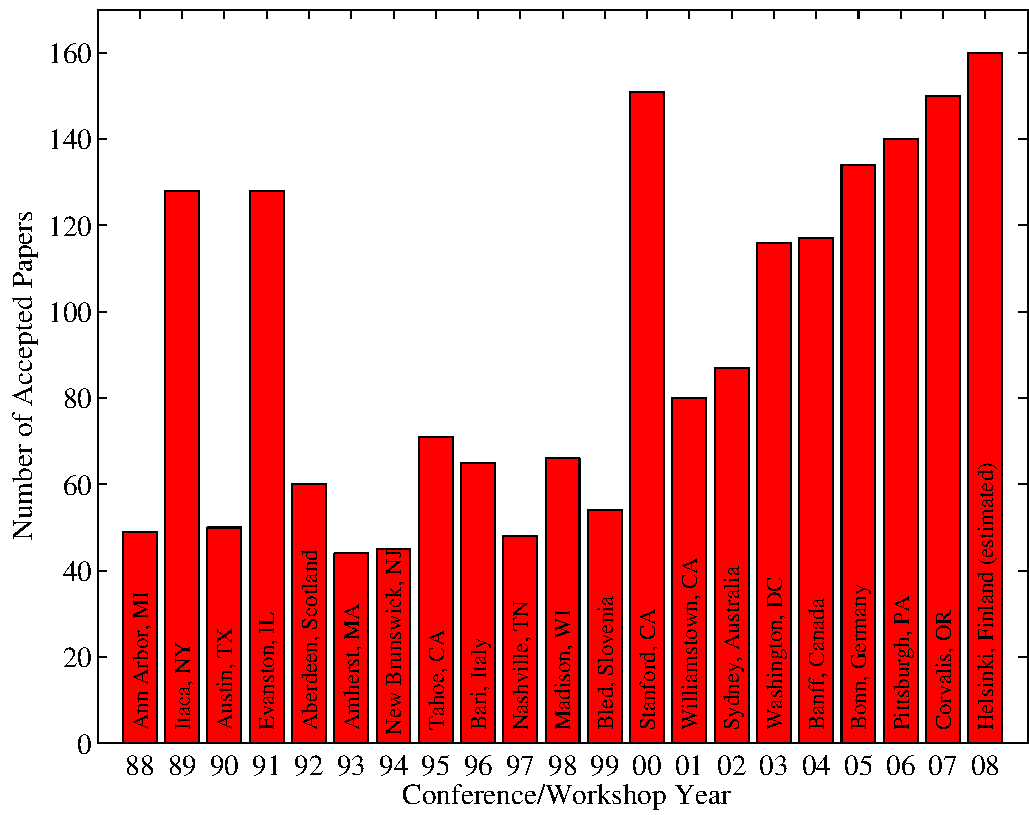
\includegraphics[width=\columnwidth]{icml_numpapers}}
\caption{Historical locations and number of accepted papers for International
Machine Learning Conferences (ICML 1993 -- ICML 2008) and International
Workshops on Machine Learning (ML 1988 -- ML 1992). At the time this figure was
produced, the number of accepted papers for ICML 2008 was unknown and instead
estimated.}
\label{icml-historical}
\end{center}
\vskip -0.2in
\end{figure}

\subsection{Figures}

You may want to include figures in the paper to illustrate
your approach and results. Such artwork should be centered,
legible, and separated from the text. Lines should be dark and at
least 0.5~points thick for purposes of reproduction, and text should
not appear on a gray background.

Label all distinct components of each figure. If the figure takes the
form of a graph, then give a name for each axis and include a legend
that briefly describes each curve. Do not include a title inside the
figure; instead, the caption should serve this function.

Number figures sequentially, placing the figure number and caption
\emph{after} the graphics, with at least 0.1~inches of space before
the caption and 0.1~inches after it, as in
\cref{icml-historical}. The figure caption should be set in
9~point type and centered unless it runs two or more lines, in which
case it should be flush left. You may float figures to the top or
bottom of a column, and you may set wide figures across both columns
(use the environment \texttt{figure*} in \LaTeX). Always place
two-column figures at the top or bottom of the page.

\subsection{Algorithms}

If you are using \LaTeX, please use the ``algorithm'' and ``algorithmic''
environments to format pseudocode. These require
the corresponding stylefiles, algorithm.sty and
algorithmic.sty, which are supplied with this package.
\cref{alg:example} shows an example.

\begin{algorithm}[tb]
   \caption{Bubble Sort}
   \label{alg:example}
\begin{algorithmic}
   \STATE {\bfseries Input:} data $x_i$, size $m$
   \REPEAT
   \STATE Initialize $noChange = true$.
   \FOR{$i=1$ {\bfseries to} $m-1$}
   \IF{$x_i > x_{i+1}$}
   \STATE Swap $x_i$ and $x_{i+1}$
   \STATE $noChange = false$
   \ENDIF
   \ENDFOR
   \UNTIL{$noChange$ is $true$}
\end{algorithmic}
\end{algorithm}

\subsection{Tables}

You may also want to include tables that summarize material. Like
figures, these should be centered, legible, and numbered consecutively.
However, place the title \emph{above} the table with at least
0.1~inches of space before the title and the same after it, as in
\cref{sample-table}. The table title should be set in 9~point
type and centered unless it runs two or more lines, in which case it
should be flush left.

% Note use of \abovespace and \belowspace to get reasonable spacing
% above and below tabular lines.

\begin{table}[t]
\caption{Classification accuracies for naive Bayes and flexible
Bayes on various data sets.}
\label{sample-table}
\vskip 0.15in
\begin{center}
\begin{small}
\begin{sc}
\begin{tabular}{lcccr}
\toprule
Data set & Naive & Flexible & Better? \\
\midrule
Breast    & 95.9$\pm$ 0.2& 96.7$\pm$ 0.2& $\surd$ \\
Cleveland & 83.3$\pm$ 0.6& 80.0$\pm$ 0.6& $\times$\\
Glass2    & 61.9$\pm$ 1.4& 83.8$\pm$ 0.7& $\surd$ \\
Credit    & 74.8$\pm$ 0.5& 78.3$\pm$ 0.6&         \\
Horse     & 73.3$\pm$ 0.9& 69.7$\pm$ 1.0& $\times$\\
Meta      & 67.1$\pm$ 0.6& 76.5$\pm$ 0.5& $\surd$ \\
Pima      & 75.1$\pm$ 0.6& 73.9$\pm$ 0.5&         \\
Vehicle   & 44.9$\pm$ 0.6& 61.5$\pm$ 0.4& $\surd$ \\
\bottomrule
\end{tabular}
\end{sc}
\end{small}
\end{center}
\vskip -0.1in
\end{table}

Tables contain textual material, whereas figures contain graphical material.
Specify the contents of each row and column in the table's topmost
row. Again, you may float tables to a column's top or bottom, and set
wide tables across both columns. Place two-column tables at the
top or bottom of the page.

\subsection{Theorems and such}
The preferred way is to number definitions, propositions, lemmas, etc. consecutively, within sections, as shown below.
\begin{definition}
\label{def:inj}
A function $f:X \to Y$ is injective if for any $x,y\in X$ different, $f(x)\ne f(y)$.
\end{definition}
Using \cref{def:inj} we immediate get the following result:
\begin{proposition}
If $f$ is injective mapping a set $X$ to another set $Y$, 
the cardinality of $Y$ is at least as large as that of $X$
\end{proposition}
\begin{proof} 
Left as an exercise to the reader. 
\end{proof}
\cref{lem:usefullemma} stated next will prove to be useful.
\begin{lemma}
\label{lem:usefullemma}
For any $f:X \to Y$ and $g:Y\to Z$ injective functions, $f \circ g$ is injective.
\end{lemma}
\begin{theorem}
\label{thm:bigtheorem}
If $f:X\to Y$ is bijective, the cardinality of $X$ and $Y$ are the same.
\end{theorem}
An easy corollary of \cref{thm:bigtheorem} is the following:
\begin{corollary}
If $f:X\to Y$ is bijective, 
the cardinality of $X$ is at least as large as that of $Y$.
\end{corollary}
\begin{assumption}
The set $X$ is finite.
\label{ass:xfinite}
\end{assumption}
\begin{remark}
According to some, it is only the finite case (cf. \cref{ass:xfinite}) that is interesting.
\end{remark}
%restatable

\subsection{Citations and References}

Please use APA reference format regardless of your formatter
or word processor. If you rely on the \LaTeX\/ bibliographic
facility, use \texttt{natbib.sty} and \texttt{icml2025.bst}
included in the style-file package to obtain this format.

Citations within the text should include the authors' last names and
year. If the authors' names are included in the sentence, place only
the year in parentheses, for example when referencing Arthur Samuel's
pioneering work \yrcite{Samuel59}. Otherwise place the entire
reference in parentheses with the authors and year separated by a
comma \cite{Samuel59}. List multiple references separated by
semicolons \cite{kearns89,Samuel59,mitchell80}. Use the `et~al.'
construct only for citations with three or more authors or after
listing all authors to a publication in an earlier reference \cite{MachineLearningI}.

Authors should cite their own work in the third person
in the initial version of their paper submitted for blind review.
Please refer to \cref{author info} for detailed instructions on how to
cite your own papers.

Use an unnumbered first-level section heading for the references, and use a
hanging indent style, with the first line of the reference flush against the
left margin and subsequent lines indented by 10 points. The references at the
end of this document give examples for journal articles \cite{Samuel59},
conference publications \cite{langley00}, book chapters \cite{Newell81}, books
\cite{DudaHart2nd}, edited volumes \cite{MachineLearningI}, technical reports
\cite{mitchell80}, and dissertations \cite{kearns89}.

Alphabetize references by the surnames of the first authors, with
single author entries preceding multiple author entries. Order
references for the same authors by year of publication, with the
earliest first. Make sure that each reference includes all relevant
information (e.g., page numbers).

Please put some effort into making references complete, presentable, and
consistent, e.g. use the actual current name of authors.
If using bibtex, please protect capital letters of names and
abbreviations in titles, for example, use \{B\}ayesian or \{L\}ipschitz
in your .bib file.

\section*{Accessibility}
Authors are kindly asked to make their submissions as accessible as possible for everyone including people with disabilities and sensory or neurological differences.
Tips of how to achieve this and what to pay attention to will be provided on the conference website \url{http://icml.cc/}.

\section*{Software and Data}

If a paper is accepted, we strongly encourage the publication of software and data with the
camera-ready version of the paper whenever appropriate. This can be
done by including a URL in the camera-ready copy. However, \textbf{do not}
include URLs that reveal your institution or identity in your
submission for review. Instead, provide an anonymous URL or upload
the material as ``Supplementary Material'' into the OpenReview reviewing
system. Note that reviewers are not required to look at this material
when writing their review.

% Acknowledgements should only appear in the accepted version.
\section*{Acknowledgements}

\textbf{Do not} include acknowledgements in the initial version of
the paper submitted for blind review.

If a paper is accepted, the final camera-ready version can (and
usually should) include acknowledgements.  Such acknowledgements
should be placed at the end of the section, in an unnumbered section
that does not count towards the paper page limit. Typically, this will 
include thanks to reviewers who gave useful comments, to colleagues 
who contributed to the ideas, and to funding agencies and corporate 
sponsors that provided financial support.

\section*{Impact Statement}

Authors are \textbf{required} to include a statement of the potential 
broader impact of their work, including its ethical aspects and future 
societal consequences. This statement should be in an unnumbered 
section at the end of the paper (co-located with Acknowledgements -- 
the two may appear in either order, but both must be before References), 
and does not count toward the paper page limit. In many cases, where 
the ethical impacts and expected societal implications are those that 
are well established when advancing the field of Machine Learning, 
substantial discussion is not required, and a simple statement such 
as the following will suffice:

``This paper presents work whose goal is to advance the field of 
Machine Learning. There are many potential societal consequences 
of our work, none which we feel must be specifically highlighted here.''

The above statement can be used verbatim in such cases, but we 
encourage authors to think about whether there is content which does 
warrant further discussion, as this statement will be apparent if the 
paper is later flagged for ethics review.


% In the unusual situation where you want a paper to appear in the
% references without citing it in the main text, use \nocite
\nocite{langley00}

\bibliography{example_paper}
\bibliographystyle{icml2025}


%%%%%%%%%%%%%%%%%%%%%%%%%%%%%%%%%%%%%%%%%%%%%%%%%%%%%%%%%%%%%%%%%%%%%%%%%%%%%%%
%%%%%%%%%%%%%%%%%%%%%%%%%%%%%%%%%%%%%%%%%%%%%%%%%%%%%%%%%%%%%%%%%%%%%%%%%%%%%%%
% APPENDIX
%%%%%%%%%%%%%%%%%%%%%%%%%%%%%%%%%%%%%%%%%%%%%%%%%%%%%%%%%%%%%%%%%%%%%%%%%%%%%%%
%%%%%%%%%%%%%%%%%%%%%%%%%%%%%%%%%%%%%%%%%%%%%%%%%%%%%%%%%%%%%%%%%%%%%%%%%%%%%%%
\newpage
\appendix
\onecolumn

\section{Frequency Domain Analysis}

\section{Experimental Hyperparameters}

\section{MT Bench Case Study}

\section{Proof of Rank Increasement}




\section{Rank Increasement Analysis}
\label{appendix:rank_increasement}




\begin{theorem}[ under nontrivial frequency masking]
\label{thm:rank_increasement}
Let $\mathbb{K}$ be either $\mathbb{R}$ or $\mathbb{C}$, denoting respectively the field of real or complex numbers. 
Let $\mW_{UV} = \sum_{i=1}^r \mU_i \mV_i^\top$ with $\mU_i\in\mathbb{K}^m$ and $\mV_i\in\mathbb{K}^n$ (so $\operatorname{rank}(\mW_{UV})\le r$). 
Let $\mM_t\in\mathbb{C}^{m\times n}$ be a frequency-domain mask and define its inverse DFT 
$h = \mathcal{F}^{-1}(\mM_t)\in\mathbb{C}^{m\times n}$, interpreted as the corresponding spatial convolution kernel. 

Assume that $h$ has finite support on $t$ distinct circular shifts, i.e.
\begin{align}
h = \sum_{k=1}^{t} \alpha_k\, S_{s_k,t_k}(\Delta),
\end{align}
where $\alpha_k\in\mathbb{C}\setminus\{0\}$, 
$\Delta$ denotes the Kronecker delta at the origin, 
and $S_{s,t}:\mathbb{K}^{m\times n}\!\to\!\mathbb{K}^{m\times n}$ denotes the two-dimensional circular shift operator defined by
\begin{align}
  [S_{s,t}(\mX)]_{i,j} = \mX_{(i-s)\bmod m,\,(j-t)\bmod n}.
\end{align}
For a vector $\mU\in\mathbb{K}^m$, we define $S_s(\mU)\in\mathbb{K}^m$ analogously as the circular shift by $s$ along its entries, 
so that $S_{s,t}(\mU \mV^\top) = S_s(\mU)\,S_t(\mV)^\top$.

Then the frequency-masked transform of $\mW_{UV}$ satisfies
\begin{align}
\mathcal{T}_{\mM_t}(\mW_{UV})
  = \sum_{k=1}^{t} \alpha_k\, S_{s_k,t_k}(\mW_{UV})
  = \sum_{i=1}^{r}\sum_{k=1}^{t} \alpha_k\, S_{s_k}(\mU_i)\,S_{t_k}(\mV_i)^\top.
\end{align}

Suppose further that the following \emph{nondegeneracy (genericity) conditions} hold:
\begin{enumerate}
\item For each $i$, the set of shifted vectors $\{S_{s_k}(\mU_i)\}_{k=1}^{t}$ is linearly independent over $\mathbb{K}$ (or at least spans a $t_i$-dimensional subspace with $t_i\ge 2$), and similarly $\{S_{t_k}(\mV_i)\}_{k=1}^{t}$ are in general position.
\item The families $\{S_{s_k}(\mU_i)\}_{i,k}$ and $\{S_{t_k}(\mV_i)\}_{i,k}$ corresponding to different $i$ are in general position, i.e. their Kruskal ranks satisfy the usual generic full-rank condition.\footnote{That is, for an open dense subset of $(\mU_i,\mV_i)$ in $\mathbb{K}^{m\times r}\times\mathbb{K}^{n\times r}$ the set of rank--1 outer products $\{S_{s_k}(\mU_i)S_{t_k}(\mV_i)^\top\}_{i,k}$ is linearly independent up to the ambient limit.}
\end{enumerate}
Then generically
\begin{align}
\operatorname{rank}\!\big(\mathcal{T}_{\mM_t}(\mW_{UV})\big)
  = \min\!\big( rt,\; \min(m,n) \big).
\end{align}
In particular, whenever $t>1$ and the above nondegeneracy conditions are satisfied,
\begin{align}
\operatorname{rank}\!\big(\mathcal{T}_{\mM_t}(\mW_{UV})\big)
   > \operatorname{rank}(\mW_{UV}).
\end{align}
\end{theorem}

\begin{lemma}[Khatri--Rao representation and generic full rank]
\label{lem:khatri-rao}
For any $u\in\mathbb{K}^m$ and $v\in\mathbb{K}^n$,
\begin{align}
  \mathrm{vec}\!\big(S_s(u)\,S_t(v)^\top\big)
  = S_t(v)\odot S_s(u),
\end{align}
where $\odot$ denotes the columnwise Kronecker (Khatri--Rao) product.
For a collection $\{S_{s_k}(\mU_i)S_{t_k}(\mV_i)^\top\}_{i=1,\dots,r;\,k=1,\dots,t}$,
define the matrix
\begin{align}
A := \big[\,S_{t_1}(\mV_1)\!\odot\!S_{s_1}(\mU_1),~
   S_{t_2}(\mV_1)\!\odot\!S_{s_2}(\mU_1),~
   \dots,~
   S_{t_t}(\mV_r)\!\odot\!S_{s_t}(\mU_r)\,\big]
   \in\mathbb{K}^{mn\times (r t)}.
\end{align}
If $A$ has full column rank, then the corresponding rank--1 atoms 
$\{S_{s_k}(\mU_i)S_{t_k}(\mV_i)^\top\}_{i,k}$ are linearly independent, and hence
\begin{align}
  \operatorname{rank}\!\big(\mathcal{T}_{\mM_t}(\mW_{UV})\big)
  = \min(rt,\,\min(m,n)).
\end{align}
Moreover, full column rank of $A$ holds for an open dense subset of 
$(\mU_i,\mV_i)\in\mathbb{K}^{m\times r}\!\times\!\mathbb{K}^{n\times r}$,
since $\det(A^\top A)$ is a nonzero polynomial in the entries of $\mU_i,\mV_i$.
\end{lemma}

\begin{assumption}[Nondegeneracy]
\label{assump:nondegeneracy}
We assume the following conditions hold:
\begin{enumerate}%[(a)]
    \item The singular vectors $\{u_i\}_{i=1}^r$ and $\{v_i\}_{i=1}^r$ of $\mW_{UV} = \sum_{i=1}^r \mU_i \mV_i^\top$ are linearly independent, i.e.,
    \[
        \mathrm{rank}\big([\mU_1,\dots,\mU_r]\big) = r, \quad 
        \mathrm{rank}\big([\mV_1,\dots,\mV_r]\big) = r.
    \]
    \item The frequency mask $\mM_t \in \mathbb{C}^{m \times n}$ is \emph{nontrivial}, meaning that it is not proportional to the all-one matrix and contains at least one element with a distinct complex phase or magnitude, formally,
    \[
        \exists (p,q),(p',q') \text{ such that } 
        \mM_t(p,q) \neq \alpha\, \mM_t(p',q') \text{ for any } \alpha \in \mathbb{C}.
    \]
\end{enumerate}
\end{assumption}


\begin{proof}
\textbf{Step 1 (Convolution representation).} 
By the convolution theorem, multiplication by $\mM_t$ in the frequency domain corresponds to circular convolution by its inverse DFT $h$ in the spatial domain:
\begin{align}
\mathcal{T}_{\mM_t}(\mW_{UV}) = h \star_{\mathrm{circ}} \mW_{UV}.
\end{align}
If $h$ is supported on $t$ distinct shifts, i.e.
$h=\sum_{k=1}^t \alpha_k S_{s_k,t_k}(\Delta)$,
then by linearity of convolution,
\begin{align}
h\star_{\mathrm{circ}} \mW_{UV}
  = \sum_{k=1}^t \alpha_k\, S_{s_k,t_k}(\mW_{UV}),
\end{align}
where $S_{s_k,t_k}(\mW_{UV})$ denotes the circularly shifted copy of $\mW_{UV}$ by $(s_k,t_k)$.

\textbf{Step 2 (Rank--1 component).} 
For a single rank--1 matrix $\mW_{UV}=\mU \mV^\top$,
\begin{align}
\mathcal{T}_{\mM_t}(\mU \mV^\top)
  = \sum_{k=1}^t \alpha_k\, S_{s_k}(\mU)\,S_{t_k}(\mV)^\top.
\end{align}
Each term is rank--1. 
If the family of shifted vectors $\{S_{s_k}(\mU)\}$ is linearly independent and the shifted $\{S_{t_k}(\mV)\}$ are in general position, then the $t$ outer products are generically linearly independent (up to $\min(m,n)$). 
Hence the rank of the resulting sum equals $\min(t,\min(m,n))$ for generic parameters.

\textbf{Step 3 (General rank--$r$ case).}
For $\mW_{UV}=\sum_{i=1}^r \mU_i \mV_i^\top$,
\begin{align}
\mathcal{T}_{\mM_t}(\mW_{UV})
  &= \sum_{i=1}^r \mathcal{T}_{\mM_t}(\mU_i \mV_i^\top)
   = \sum_{i=1}^r \sum_{k=1}^t \alpha_k\, S_{s_k}(\mU_i)\,S_{t_k}(\mV_i)^\top.
\end{align}
The right-hand side is a linear combination of $r\!\cdot\!t$ rank--1 atoms. 
Under assumption~\ref{assump:nondegeneracy}, the set of these rank--1 atoms is generically linearly independent up to the ambient limit, so the rank equals
\begin{align}
\operatorname{rank}\big(\mathcal{T}_{\mM_t}(\mW_{UV})\big)
  = \min(r t, \min(m,n)).
\end{align}


\textbf{Step 4 (Existence of such masks).}
For any prescribed $t>1$, one can explicitly construct $h=\sum_{k=1}^t \alpha_k S_{s_k,t_k}(\Delta)$ with distinct shifts $(s_k,t_k)$ and nonzero $\alpha_k$, 
and define $\mM_t = \mathcal{F}(h)$. 
For generic $\mU_i,\mV_i$, the corresponding transform $\mathcal{T}_{\mM_t}$ then strictly increases rank.

\textbf{Step 5 (Field consistency).}
If all $\alpha_k$, $\mU_i$, $\mV_i$ are real, the argument holds over $\mathbb{R}$; 
if some $\alpha_k$ are complex, rank is interpreted over $\mathbb{C}$. 
Either way, the statement remains valid with the appropriate field.
\end{proof}

\begin{remark}[Discussion and genericity]
\begin{enumerate}
\item 
The assumption that $h$ is a finite sum of shifted deltas is a constructive special case. 
More generally, if $h$ has $t$ well-separated dominant coefficients (effective support), the same argument applies approximately, replacing exact rank by numerical rank determined by the singular values.

\item 
The conclusion is \emph{generic}: for an open dense subset of $(\mU_i,\mV_i,\alpha_k)$ in $\mathbb{K}^{m\times r}\!\times\!\mathbb{K}^{n\times r}\!\times\!(\mathbb{C}\setminus\{0\})^t$, 
the linear independence of the rank--1 atoms 
$\{S_{s_k}(\mU_i)S_{t_k}(\mV_i)^\top\}_{i,k}$ holds, and the rank achieves the upper bound $\min(r t,\min(m,n))$. 
Degenerate counterexamples occur if $\mU_i$ or $\mV_i$ are shift-invariant (e.g. constant or periodic), in which case the rank may fail to increase.

\item 
In vectorized operator form, 
\begin{align}
\mathrm{vec}\!\big(\mathcal{T}_{\mM_t}(\mW_{UV})\big)
   = C_{\mM_t}\,\mathrm{vec}(\mW_{UV}),
   \quad C_{\mM_t} := \mathcal{F}^{-1} \operatorname{diag}(\mathrm{vec}(\mM_t)) \mathcal{F}.
\end{align}
The operator $C_{\mM_t}$ has rank equal to the number of nonzero entries in $\mM_t$.
If all frequencies are retained ($\mM_t$ has no zeros), $C_{\mM_t}$ is invertible (full rank).
When $\mM_t$ is a nontrivial mask (some zeros), $C_{\mM_t}$ is not full rank, yet it can still map a low-rank $\mW_{UV}$ to a higher-rank output 
because the linear mixing introduced by the circular shifts breaks the low-rank structure.
\end{enumerate}
\end{remark}

\section{ADD}


\noindent\textbf{Genericity clarification.}
Condition~(b) may be stated equivalently as: 
the matrix $A$ defined in Lemma~\ref{lem:khatri-rao} has full column rank.
Equivalently, for all nonzero coefficient tensors $\{\beta_{i,k}\}$,
\begin{align}
  \sum_{i=1}^r\sum_{k=1}^t
     \beta_{i,k}\,S_{s_k}(\mU_i)\,S_{t_k}(\mV_i)^\top = 0
  \quad\Longrightarrow\quad
  \beta_{i,k}=0~\forall i,k.
\end{align}
This condition is satisfied for an open dense set of $(\mU_i,\mV_i)$,
so the rank formula holds \emph{generically}.


% \section{Rank Increasement Prev. Ver.}
% \textbf{Step 1 (Convolution representation of the masked transform).}

% Let $\mW_{UV}\in\mathbb{R}^{m\times n}$. Denote by $\mathcal{F}:\mathbb{C}^{m\times n}\to\mathbb{C}^{m\times n}$ the 2D DFT acting on the matrix entries (we use the convention that $\mathcal{F}$ is invertible and $\mathcal{F}^{-1}$ is the inverse DFT). For a frequency-domain mask $\mM_t\in\mathbb{C}^{m\times n}$ define the frequency-domain multiplication operator for task $t$
% \begin{align}
% \mathcal{T}_{\mM_t}(\mW_{UV}) \coloneqq \mathcal{F}^{-1}\big(\mM_t \odot \mathcal{F}(\mW_{UV})\big),
% \end{align}
% where $\odot$ denotes elementwise (Hadamard) product. We will study $\mathcal{T}_{\mM_t}(\mW_{UV})$ when $\mW_{UV}=\mU\mV^\top$ with $\mU\in\mathbb{R}^{m\times r}, \mV\in\mathbb{R}^{n\times r}$ (so $\operatorname{rank}(\mW_{UV})\le r$).

% Observe that the elementwise multiplication in the frequency domain is equivalent to a circular convolution in the spatial domain. Specifically, there exists a kernel $h = \mathcal{F}^{-1}(\mM_t) \in \mathbb{C}^{m\times n}$, representing the inverse discrete Fourier transform (DFT) of the mask $\mM_t$, such that
% \begin{align}
% \mathcal{T}_{\mM_t}(\mW_{UV}) = h \star_{\mathrm{circ}} \mW_{UV},
% \end{align}
% where $\star_{\mathrm{circ}}$ denotes 2D circular convolution (convolution performed with wrap-around on both dimensions). In other words, $\mM_t$ determines $h$, and the frequency-domain masking by $\mM_t$ is equivalent to a circular convolution with $h$ in the spatial domain. The following theorem makes precise how the rank can increase.

% \begin{theorem}[Rank increase under nontrivial frequency masking]
% \label{thm:rank_increase}




% Let $\mW_{UV}=\sum_{i=1}^r \mU_i \mV_i^\top$ with $\mU_i\in\mathbb{R}^m$, $\mV_i\in\mathbb{R}^n$ (so $\operatorname{rank}(\mW_{UV})\le r$). Let $\mM_t$ be a frequency mask and write $h=\mathcal{F}^{-1}(\mM_t)\in\mathbb{C}^{m\times n}$ for its inverse DFT (the spatial kernel). Suppose $h$ can be written as a finite sum of $t$ distinct shifted deltas (i.e. it is supported on $t$ distinct circular shifts):
% \begin{align}
% h = \sum_{k=1}^{t} \alpha_k S_{s_k,t_k}(\Delta),
% \end{align}
% where $\alpha_k\in\mathbb{C}\setminus\{0\}$, $S_{s_k,t_k}$ denotes the circular shift operator by $(s_k,t_k)$ in the two dimensions, and $\Delta$ is the Kronecker delta at the origin. (Equivalently, $h$ has exactly $t$ nonzero entries located at distinct coordinates.) Then
% \begin{align}
% \mathcal{T}_{\mM_t}(\mW_{UV}) \;=\; \sum_{k=1}^{t} \alpha_k \, S_{s_k,t_k}(\mW_{UV}).
% \end{align}
% In particular, if for each fixed $i$ the set of shifted vectors $\{\,S_{s_k} \mU_i : k=1,\dots,t\,\}$ (row-shifts of $\mU_i$) contains at least $t_i$ linearly independent vectors, and similarly the column-shifts of $\mV_i$ are in general position, then generically
% \begin{align}
% \operatorname{rank}\big(\mathcal{T}_{\mM_t}(\mW_{UV})\big) \ge \min\big( rt, \; \min(m,n) \big).
% \end{align}
% Hence, for any $X$ of rank $r$ there exist masks $M$ (equivalently kernels $h$ with $t\!>\!1$ nonzero shifts) such that
% \begin{align}
% \operatorname{rank}\big(\mathcal{T}_{\mM_t}(\mW_{UV})\big) > \operatorname{rank}(\mW_{UV}).
% \end{align}
% \end{theorem}

% \begin{proof}
% Step 1 (convolution expansion). Since $h=\mathcal{F}^{-1}(M)$, by linearity of DFT/IDFT and the convolution theorem we have for any matrix $\mW_{UV}$,
% \begin{align}
% \mathcal{T}_{\mM_t}(\mW_{UV}) = h \star_{\mathrm{circ}} \mW_{UV}.
% \end{align}
% If $h$ is supported on $t$ distinct circular shifts (i.e. has nonzero entries at exactly $t$ coordinates), then the circular convolution with $\mW_{UV}$ reduces to a finite sum of shifted copies of $X$ weighted by those kernel entries. Writing the shifts explicitly,
% \begin{align}
% h=\sum_{k=1}^t \alpha_k S_{s_k,t_k}(\Delta)
% \quad\Longrightarrow\quad
% h\star_{\mathrm{circ}} \mW_{UV} = \sum_{k=1}^t \alpha_k\, S_{s_k,t_k}(\mW_{UV}),
% \end{align}
% where $S_{s_k,t_k}(\mW_{UV})$ denotes $\mW_{UV}$ circularly shifted by $(s_k,t_k)$ (shift of rows by $s_k$ and columns by $t_k$).

% Step 2 (apply to rank-$1$ atoms). For a rank--1 matrix $\mW_{UV} = \mU \mV^\top$ we then get
% \begin{align}
% \mathcal{T}_{\mM_t}(\mU \mV^\top) = \sum_{k=1}^t \alpha_k \, S_{s_k}(\mU)\,S_{t_k}(\mV)^\top
% \end{align}
% which is an explicit sum of $t$ rank--1 matrices. If the set of row-shifted vectors $\{S_{s_k}(\mU)\}_{k=1}^t$ is linearly independent (or, more weakly, if the family of outer products produce a span of dimension $t$), then the rank of the right-hand side equals $t$ (up to the ambient dimension limit). Thus a single rank--1 atom can be mapped to a matrix of rank up to $\min(t,\min(m,n))$.

% Step 3 (general rank $r$). For general $\mW_{UV}=\sum_{i=1}^r \mU_i \mV_i^\top$, by linearity
% \begin{align}
% \mathcal{T}_{\mM_t}(\mW_{UV}) = \sum_{i=1}^r \sum_{k=1}^t \alpha_k \, S_{s_k}(\mU_i)\,S_{t_k}(\mV_i)^\top,
% \end{align}
% a sum of $r\cdot t$ rank--1 terms. The rank of this sum is bounded above by $\min(r\cdot t,\min(m,n))$ and (by standard genericity arguments) is equal to that upper bound for a generic choice of the vectors $\{\mU_i\}$, $\{\mV_i\}$ and nondegenerate coefficients $\{\alpha_k\}$. Consequently, whenever $t>1$ and the shifts produce new independent components (i.e. the shifted vectors are not all collinear), the rank strictly increases compared to the original rank $\le r$.
% \begin{align}
% \operatorname{rank}\big(\mathcal{T}_{\mM_t}(\mW_{UV})\big) \ge \min\big( r\cdot t, \; \min(m,n) \big).
% \end{align}
% Step 4 (existence). The final statement follows because one can always choose a mask $M$ whose inverse DFT $h$ is (for example) the sum of $t$ distinct Kronecker deltas with nonzero weights; such an $M$ exists (take $M=\mathcal{F}(h)$). For such masks, provided the data vectors are not in a degenerate alignment, the rank strictly increases.

% This completes the proof.
% \end{proof}

% \begin{remark}
% \begin{enumerate}
% \item The hypothesis that $h$ is a sum of a finite number of shifted deltas is only one convenient constructive case; more generally if $h$ has effective support on $t$ well-separated locations (or can be approximated by such), the same reasoning applies approximately.
% \item The result is \emph{generic} in the sense that for an open dense set of masks $\mM$ (or of input factors $\mU,\mV$) the inequality $\operatorname{rank}(\mathcal{T}_{\mM_t}(\mU\mV))>\operatorname{rank}(\mU\mV)$ holds whenever the spatial kernel has $t>1$ effective shifts. Degenerate counterexamples exist (e.g. if $\mU$ or $\mV$ have shift-invariant structure that cancels the shifts), so one must state the nondegeneracy assumptions as above.
% \item In operator notation: vec$(\mathcal{T}_{\mM_t}(\mW_{UV})) = C_M\,\mathrm{vec}(X)$ where $C_M=\mathcal{F}^{-1}\operatorname{diag}(\mathrm{vec}(\mM))\mathcal{F}$ is a linear operator; for generic $\mM$ the operator $C_{\mM}$ is full (or high) rank, so it does not preserve low rank of $X$.
% \end{enumerate}
% \end{remark}

\end{document}


% This document was modified from the file originally made available by
% Pat Langley and Andrea Danyluk for ICML-2K. This version was created
% by Iain Murray in 2018, and modified by Alexandre Bouchard in
% 2019 and 2021 and by Csaba Szepesvari, Gang Niu and Sivan Sabato in 2022.
% Modified again in 2023 and 2024 by Sivan Sabato and Jonathan Scarlett.
% Previous contributors include Dan Roy, Lise Getoor and Tobias
% Scheffer, which was slightly modified from the 2010 version by
% Thorsten Joachims & Johannes Fuernkranz, slightly modified from the
% 2009 version by Kiri Wagstaff and Sam Roweis's 2008 version, which is
% slightly modified from Prasad Tadepalli's 2007 version which is a
% lightly changed version of the previous year's version by Andrew
% Moore, which was in turn edited from those of Kristian Kersting and
% Codrina Lauth. Alex Smola contributed to the algorithmic style files.
% 用LoRA做multitask learning, \mathcal{S}_t = \mathrm{span}\left\{ U \cdot \mathcal{F}^{-1}\!\big(M_t \odot Z \big) : Z \in \mathbb{R}^{r \times d} \right\}. 先用multitask learning學好U和V,然後請給我一個方法規定每個subtask的mask M和scaling vector G。讓各個subtask互相不幹擾,而且單個任務的效能接近單任務訓練。

% 現在我有一個lora模組UV。UV是通過multitask learning學習出來的,接下來我要給他做FFT,然後用一個mask來選擇10%的頻率,然後再加一個額外的頻率來微調到下遊任務。請幫我設計一個演算法,實現mask如何選擇最合適的頻率,以及額外頻率應該加在頻譜的哪些位置上

% 現在我有一個lora模組UV。 y= (W + IFFT(M_t \odot FFT(UV)))x + b,幫我用可以寫在ICML論文裡面的latex格式,嚴謹證明IFFT(M_t \odot FFT(UV))的rank要大於UV


